\documentclass{handout}


\SetCourseTitle{ECE495: Fundamentals of Robotics Research}
\SetHandoutTitle{Module 0 - Intro \& GIT}
%\SetDueDate{8 Sep at 0715 (via Gradescope)}
%\ShowAllBlanks

%\showsoln \setsolncolor{red}

\newlist{todolist}{itemize}{2}
\setlist[todolist]{label=$\square$}
\usepackage{pifont}
\newcommand{\cmark}{\ding{51}}%
\newcommand{\xmark}{\ding{55}}%
\newcommand{\done}{\rlap{$\square$}{\raisebox{2pt}{\large\hspace{1pt}\cmark}}%
	\hspace{-2.5pt}}
\newcommand{\wontfix}{\rlap{$\square$}{\large\hspace{1pt}\xmark}}

\usepackage{hyperref}

\definecolor{code}{HTML}{ECF8F4}
\definecolor{comments}{HTML}{5269A5}

\usepackage[T1]{fontenc}
\lstset{%
	language=bash, upquote=true,
	otherkeywords={rostopic, rosnode, rosrun, roscore, cd, sudo, nano, echo, mkdir, touch, chmod, catkin\_make, rosmsg, rosservice, catkin\_create\_pkg, rospack, ssh, rosed},
	showspaces=false, showtabs=false, showstringspaces=false, upquote=true, tabsize=4,
	literate={~} {$\sim$}{1},
	showstringspaces=false,
	xleftmargin=0.06\textwidth,
	linewidth=0.99\textwidth,
	columns=fullflexible,
	backgroundcolor=\color{code},
	keepspaces=true,
	breaklines=true,
	basicstyle={\small\fontfamily{fvm}\fontseries{m}\selectfont},
	keywordstyle={\small\fontfamily{fvm}\fontseries{b}\selectfont},
	commentstyle={\color{comments}\small\fontfamily{fvm}\itshape\selectfont},
	belowcaptionskip=10pt,
	float=h
}

\graphicspath{{./figs/}}


\begin{document}
\maketitle

\begin{figure}[H]
	\centering
	
\includegraphics[width=.75\textwidth]{Cover.PNG}
\end{figure}

\textbf{Lesson Objectives:}
\begin{enumerate} \setlength\itemsep{0em}
	\item Learn fundamental concepts of ROS.
	\item Setup GIT repositories on both the master and the robot.
\end{enumerate}

\textbf{Agenda:}
\begin{enumerate} \setlength\itemsep{0em}
	\item Syllabus review.
	\item ROS overview.
	\item Setting up GIT repositories.
\end{enumerate}

\newpage
\clearpage
\pagebreak

\section{Setting up GIT repositories.}
\subsection{Create a repo within the GitHub Classroom:}
\begin{enumerate}
	\item Browse to \url{github.com} and create a GitHub account if you do not already have one. It is useful if your username is something that identifies you (e.g. bneff1013).
	\item \textbf{\underline{One student per group}} do the following on your personal computer: 
	\begin{enumerate}

	\item Browse to \url{https://classroom.github.com/a/woMT5_c1}.
	\item Select "Accept this assignment"
	\item You may need to hit refresh, but eventually it will provide you a link to the repository.
	\item Browse to your repository.
	\item Note the url for your repository (save this link, it is the best way to check if your repo is updated).
	\item Go to Settings -> Manage access -> and "Invite teams or people".
	\item Provide access to your team member using their GitHub user name.
	\item Browse to \url{https://classroom.github.com/a/58EyOwaM} and repeat steps b-g.
		\end{enumerate}
\end{enumerate}

\subsection{Enable SSH connection to your GitHub account}
\begin{enumerate}
	\item Open a terminal on your master (ctrl+alt+t).
	\item The same student as step 1.1.2 do the following:
	\begin{enumerate}
		\item Generate a new SSH key, substituting your GitHub email address:
\begin{lstlisting}[language=bash]
dfec@masterX:~$ ssh-keygen -t ed25519 -C "your_email@example.com"
\end{lstlisting}
		\item When you're prompted to "Enter a file in which to save the key," click enter.
		\item At the prompt, type a secure passphrase.
		\item Start the ssh-agent in the background and add your SSH private key to the ssh-agent:
\begin{lstlisting}[language=bash]
dfec@masterX:~$ eval "$(ssh-agent -s)"
dfec@masterX:~$ ssh-add ~/.ssh/id_ed25519
\end{lstlisting}
		\item Open the public key:
\begin{lstlisting}[language=bash]
dfec@masterX:~$ nano ~/.ssh/id_ed25519.pub
\end{lstlisting}
		\item Select the contents of the file (maximize the window and ensure it has your GIT email at the end), right click, and select copy.
		\item Open a web browser and sign in to your GitHub account.
\newpage
\clearpage
\pagebreak
		\item In the upper-right corner of any page, click your profile photo, then click \textbf{Settings}
		\begin{figure}[H]
			\centering
			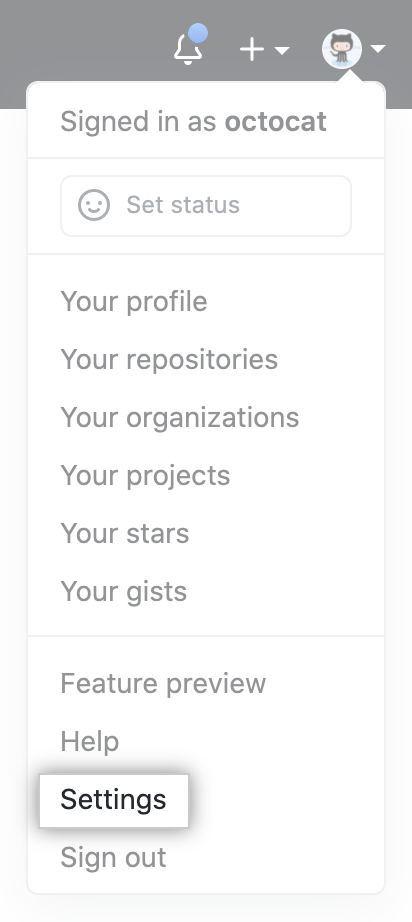
\includegraphics[width=.25\textwidth]{userbar-account-settings.PNG}
		\end{figure}

		\item In the user settings sidebar, click \textbf{SSH and GPG keys}.
		\begin{figure}[H]
			\centering
			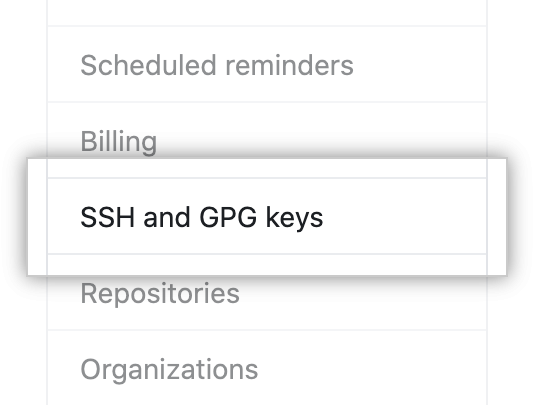
\includegraphics[width=.25\textwidth]{settings-sidebar-ssh-keys.PNG}
		\end{figure}
		\item Click \textbf{New SSH key}
		\begin{figure}[H]
			\centering
			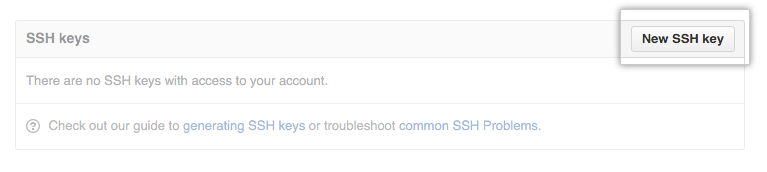
\includegraphics[width=.5\textwidth]{ssh-add-ssh-key.png}
		\end{figure}
		\item In the "Title" field, add a descriptive label for the new key, such as "MasterX".
		\item Paste your key into the "Key" field (contents of the \texttt{.pub} file).
		\item Click \textbf{Add SSH key}.
		\item If prompted, confirm your GitHub password.
		\item Create a SSH connection to your Robot (password is dfec3141):
\begin{lstlisting}[language=bash]
dfec@masterX:~$ ssh pi@robotX
\end{lstlisting}
		\item Repeat steps a-f on your robot and j-n on your master.
	\end{enumerate}
\end{enumerate}
\subsection{Clone repository to your master.}
\begin{enumerate}
\item On the master, open the \textbf{master} GitHub repository and copy your repo address using the SSH mode:
\begin{figure}[H]
	\centering
	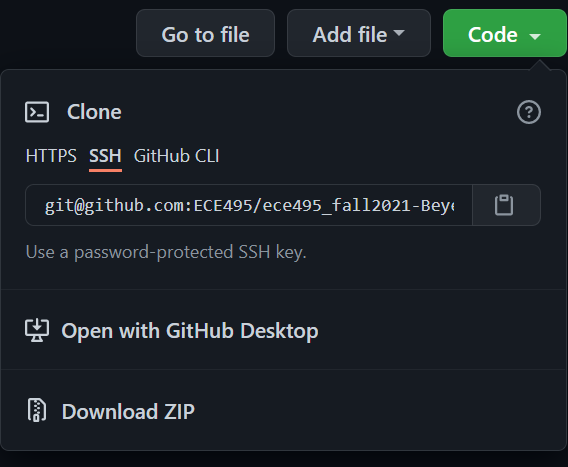
\includegraphics[width=.4\textwidth]{clone.png}
\end{figure}
\item Open a terminal and browse to your workspace source folder:
\begin{lstlisting}[language=bash]
dfec@masterX:~$ cd ~/master_ws/src/
\end{lstlisting}
\item Clone your repo using the username and password used when you generated the SSH key, replacing \textbf{USERNAME} with your GitHub username:
\begin{lstlisting}[language=bash]
dfec@masterX:~$ git clone git@github.com:ECE495/ece495_master_spring2022-USERNAME.git
\end{lstlisting}

\item Update your git email address and the last name for you and your team mate.
\begin{lstlisting}[language=bash]
dfec@masterX:~$ git config --global user.email "you@example.com"
dfec@masterX:~$ git config --global user.name "Lastname1 Lastname2"
\end{lstlisting}
\end{enumerate}

\subsection{Clone repository to your robot.}
\begin{enumerate}
	\item Create a secure shell connection to your robot:
\begin{lstlisting}[language=bash]
dfec@masterX:~$ ssh pi@robotX
\end{lstlisting}
\item Ensure you are in the ROS robot workspace src directory.
\begin{lstlisting}[language=bash]
pi@robotX:~$ cd robot_ws/src
\end{lstlisting}
	\item Clone the \textbf{robot} repository:
\begin{lstlisting}[language=bash]
dfec@masterX:~$ git clone git@github.com:ECE495/ece495_robot_spring2022-USERNAME.git
\end{lstlisting}

\item Update your git email address and the last name for you and your team mate.
\begin{lstlisting}[language=bash]
pi@robotX:~$ git config --global user.email "you@example.com"
pi@robotX:~$ git config --global user.name "Lastname1 Lastname2"
\end{lstlisting}
\end{enumerate}

\subsection{Repository Management:}
\textbf{**IMPORTANT**}: It is vital that you \textbf{ALWAYS} pull when you start working on your code on one system and \textbf{ALWAYS} push when you are done working on your code on that system.

\textbf{**MEMORIZE THESE STEPS**}:
\begin{enumerate}
	\item Pull your repo on the master (from \texttt{ece495\_master\_spring2022-USERNAME} folder):
\begin{lstlisting}[language=bash]
dfec@masterX:~$ git pull
\end{lstlisting}
	\item Complete work on the master. For example, accomplish the following:
	\begin{enumerate}
		\item Create a file in your repo (from the \texttt{ece495\_master\_spring2022-USERNAME} folder)

\begin{lstlisting}[language=bash]
dfec@masterX:~$ touch README.md
dfec@masterX:~$ nano README.md	
\end{lstlisting}

\item Copy the following to the file completing with your own information:
\begin{lstlisting}
# ECE495 Fundamentals of Robotics
## Master System
This repository stores all code for the master computer

### Team Member 1
Name:
Go by name:
Hometown:
Desired AFSC:
Clubs/IC Sports:
### Team member 2
Name:
Go by name:
Hometown:
Desired AFSC:
Clubs/IC Sports:
\end{lstlisting}
\item Hit 'ctrl+s' then 'ctrl+x' to save and exit the editor.
	\end{enumerate}
	\item Add the files that will be uploaded to your repository:
\begin{lstlisting}[language=bash]
dfec@masterX:~$ git add -A
\end{lstlisting}
	\item Commit your changes to the repository with a message:
\begin{lstlisting}[language=bash]
dfec@masterX:~$ git commit -m "Completed README on the master!"
\end{lstlisting}
	\item Push your changes to the repository:
\begin{lstlisting}[language=bash]
dfec@masterX:~$ git push
\end{lstlisting}
	\item Pull your repo on the robot
\begin{lstlisting}[language=bash]
pi@robotX:~$ git pull
\end{lstlisting}
		\item Complete work on the robot. For example, accomplish the following:
	\begin{enumerate}
		\item Create a file in your repo (from the \texttt{ece495\_robot\_spring2022-USERNAME} folder)
		
\begin{lstlisting}[language=bash]
pi@robotX:~$ touch README.md
pi@robotX:~$ nano README.md	
\end{lstlisting}
		
		\item Copy the following to the file completing with your own information:
\begin{lstlisting}
# ECE495 Fundamentals of Robotics
## Robot System
This repository stores all code for the robot computer

### Team Member 1
Name:
Go by name:
Hometown:
Desired AFSC:
Clubs/IC Sports:
### Team member 2
Name:
Go by name:
Hometown:
Desired AFSC:
Clubs/IC Sports:
\end{lstlisting}
\item Hit 'ctrl+s' then 'ctrl+x' to save and exit the editor.
	\end{enumerate}
\item Add the files that will be uploaded to your repository:
\begin{lstlisting}[language=bash]
pi@robotX:~$ git add -A
\end{lstlisting}
\item Commit your changes to the repository with a message:
\begin{lstlisting}[language=bash]
pi@robotX:~$ git commit -m "Completed README on the robot!"
\end{lstlisting}
\item Push your changes to the repository:
\begin{lstlisting}[language=bash]
pi@robotX:~$ git push
\end{lstlisting}
\end{enumerate}

\textbf{**BOTTOM LINE**}: Ensure you pull changes, make edits, and push your changes \textbf{EVERY TIME} you work on the master or robot!

\textbf{Checkpoint. Show the instructor both repositories with READMEs on the GitHub website.}

\section{Assignments.}
\begin{todolist}
	\item[\done] If you got your repo set up on both the master and the robot, then you are good to go!
\end{todolist}

\section{Next time.}
	\begin{itemize}
		\item Module 1 - ROS
	\end{itemize}

\end{document}
